\chapter{Data Acquisition and Preprocessing}\label{ch:3}

In the preceding chapter, it was shown how certain metrics can be extracted from a target scatterer using its radar response, where the values the radar produces after matched filtering and \gls{iq}-demodulation was on the form of complex \gls{iq} radar sweeps. In this chapter, we continue with describing how measurements are acquired, structured, and preprocessed. Some \gls{pcr} system settings are discussed.

\section{Data Representation}

A common representation of data acquired by multi-antenna radars is the \emph{datacube} \citep{richards_2014}. The first dimension of the datacube consists of the radar sweeps, as described in section \ref{sec:iq}. Radar sweeps are formed by estimating the time-of-flight of a returning wavelet from a target scene, as described in section \ref{sec:mf}. This process forms the shortest time frame possible with sample spacing on the picosecond scale for millimeter-wave radar, and is thus commonly referred to as the \emph{fast time} scale. New radar sweeps are acquired at a rate set by the sampling frequency. This sequence of radar sweeps form the second dimension of the datacube. Due to its much slower rate, it is aptly referred to as the \emph{slow time} scale. Finally, the last dimension is constructed from the antenna array. This representation of data acquired by radar arrays are often referenced in journal papers when describing, for instance, beam forming or Doppler processing algorithms \citep{gentile_donovan_2018}.

We are thus working with two time scales simultaneously. Previously, the variable $t$ described the fast time scale, but it will from this point be referred to as the slow time scale to accomodate for this new dimension. Instead, we will denote the fast time scale with its corresponding range. 

The \gls{pcr} system considered in this work only has a single receiving antenna, meaning it does not capture angular information, as discussed in section \ref{single_antenna}. Thus, we are left with data representing only fast and slow time dimensions. Two such systems are used in parallel, but are not synchronized to one another. This essentially means that the sensors take turn in capturing radar sweeps as opposed to listening to the same echo wavelets. Angular information is still omitted, but using two sensors, surface characteristics can be more accurately captured.

%The \gls{pcr} system considered in this work only has a single receiving antenna, generating data with only fast and slow time dimensions. Two such systems are used in parallel, but are not synchronized to one another. This essentially means that sensors take turn in capturing radar sweeps as opposed to listening to the same echo wavelets. %Thus it would be incorrect, or at least misleading, to treat these two sensors as the third dimension of a datacube which would indicate that the two sensors are synchronized. 

For our intents and purposes, we may concatenate the two discrete sensor outputs to form a \emph{data matrix}. If a radar sensor's output with fast time index $d=1...Z$ and slow time index $t=1...Q$ is described by $r(d,t)$, we form a data matrix $\mathbf{D}$ with sensors $r_1(d,t)$ and $r_2(d,t)$ through
\begin{equation}
	\mathbf{D}= 
	\begin{bmatrix}
		r_1(0,0) & r_1(1,0) & \cdots & r_1(Z,0) & r_2(0,0) & \cdots & r_2(Z,0) \\
		r_1(0,1) & r_1(1,1) & \cdots & r_1(Z,1) & r_2(0,1) & \cdots & r_2(Z,1) \\
		\vdots &  \vdots & \ddots & \vdots & \vdots & \ddots &  \vdots \\
		r_1(0,Q) & r_1(0,Q) & \cdots  & r_1(Z,Q) & r_2(0,Q) & \cdots  & r_2(Z,Q) \\
	\end{bmatrix}
	,
\end{equation}
or, more succinctly, as samples $r(n,t) = \mathbf{D}_{n,t}$ with $n=1...2Z$. Each collected data matrix is built up of $Q=50,000$ slow time samples.

\begin{figure}
	\centering
	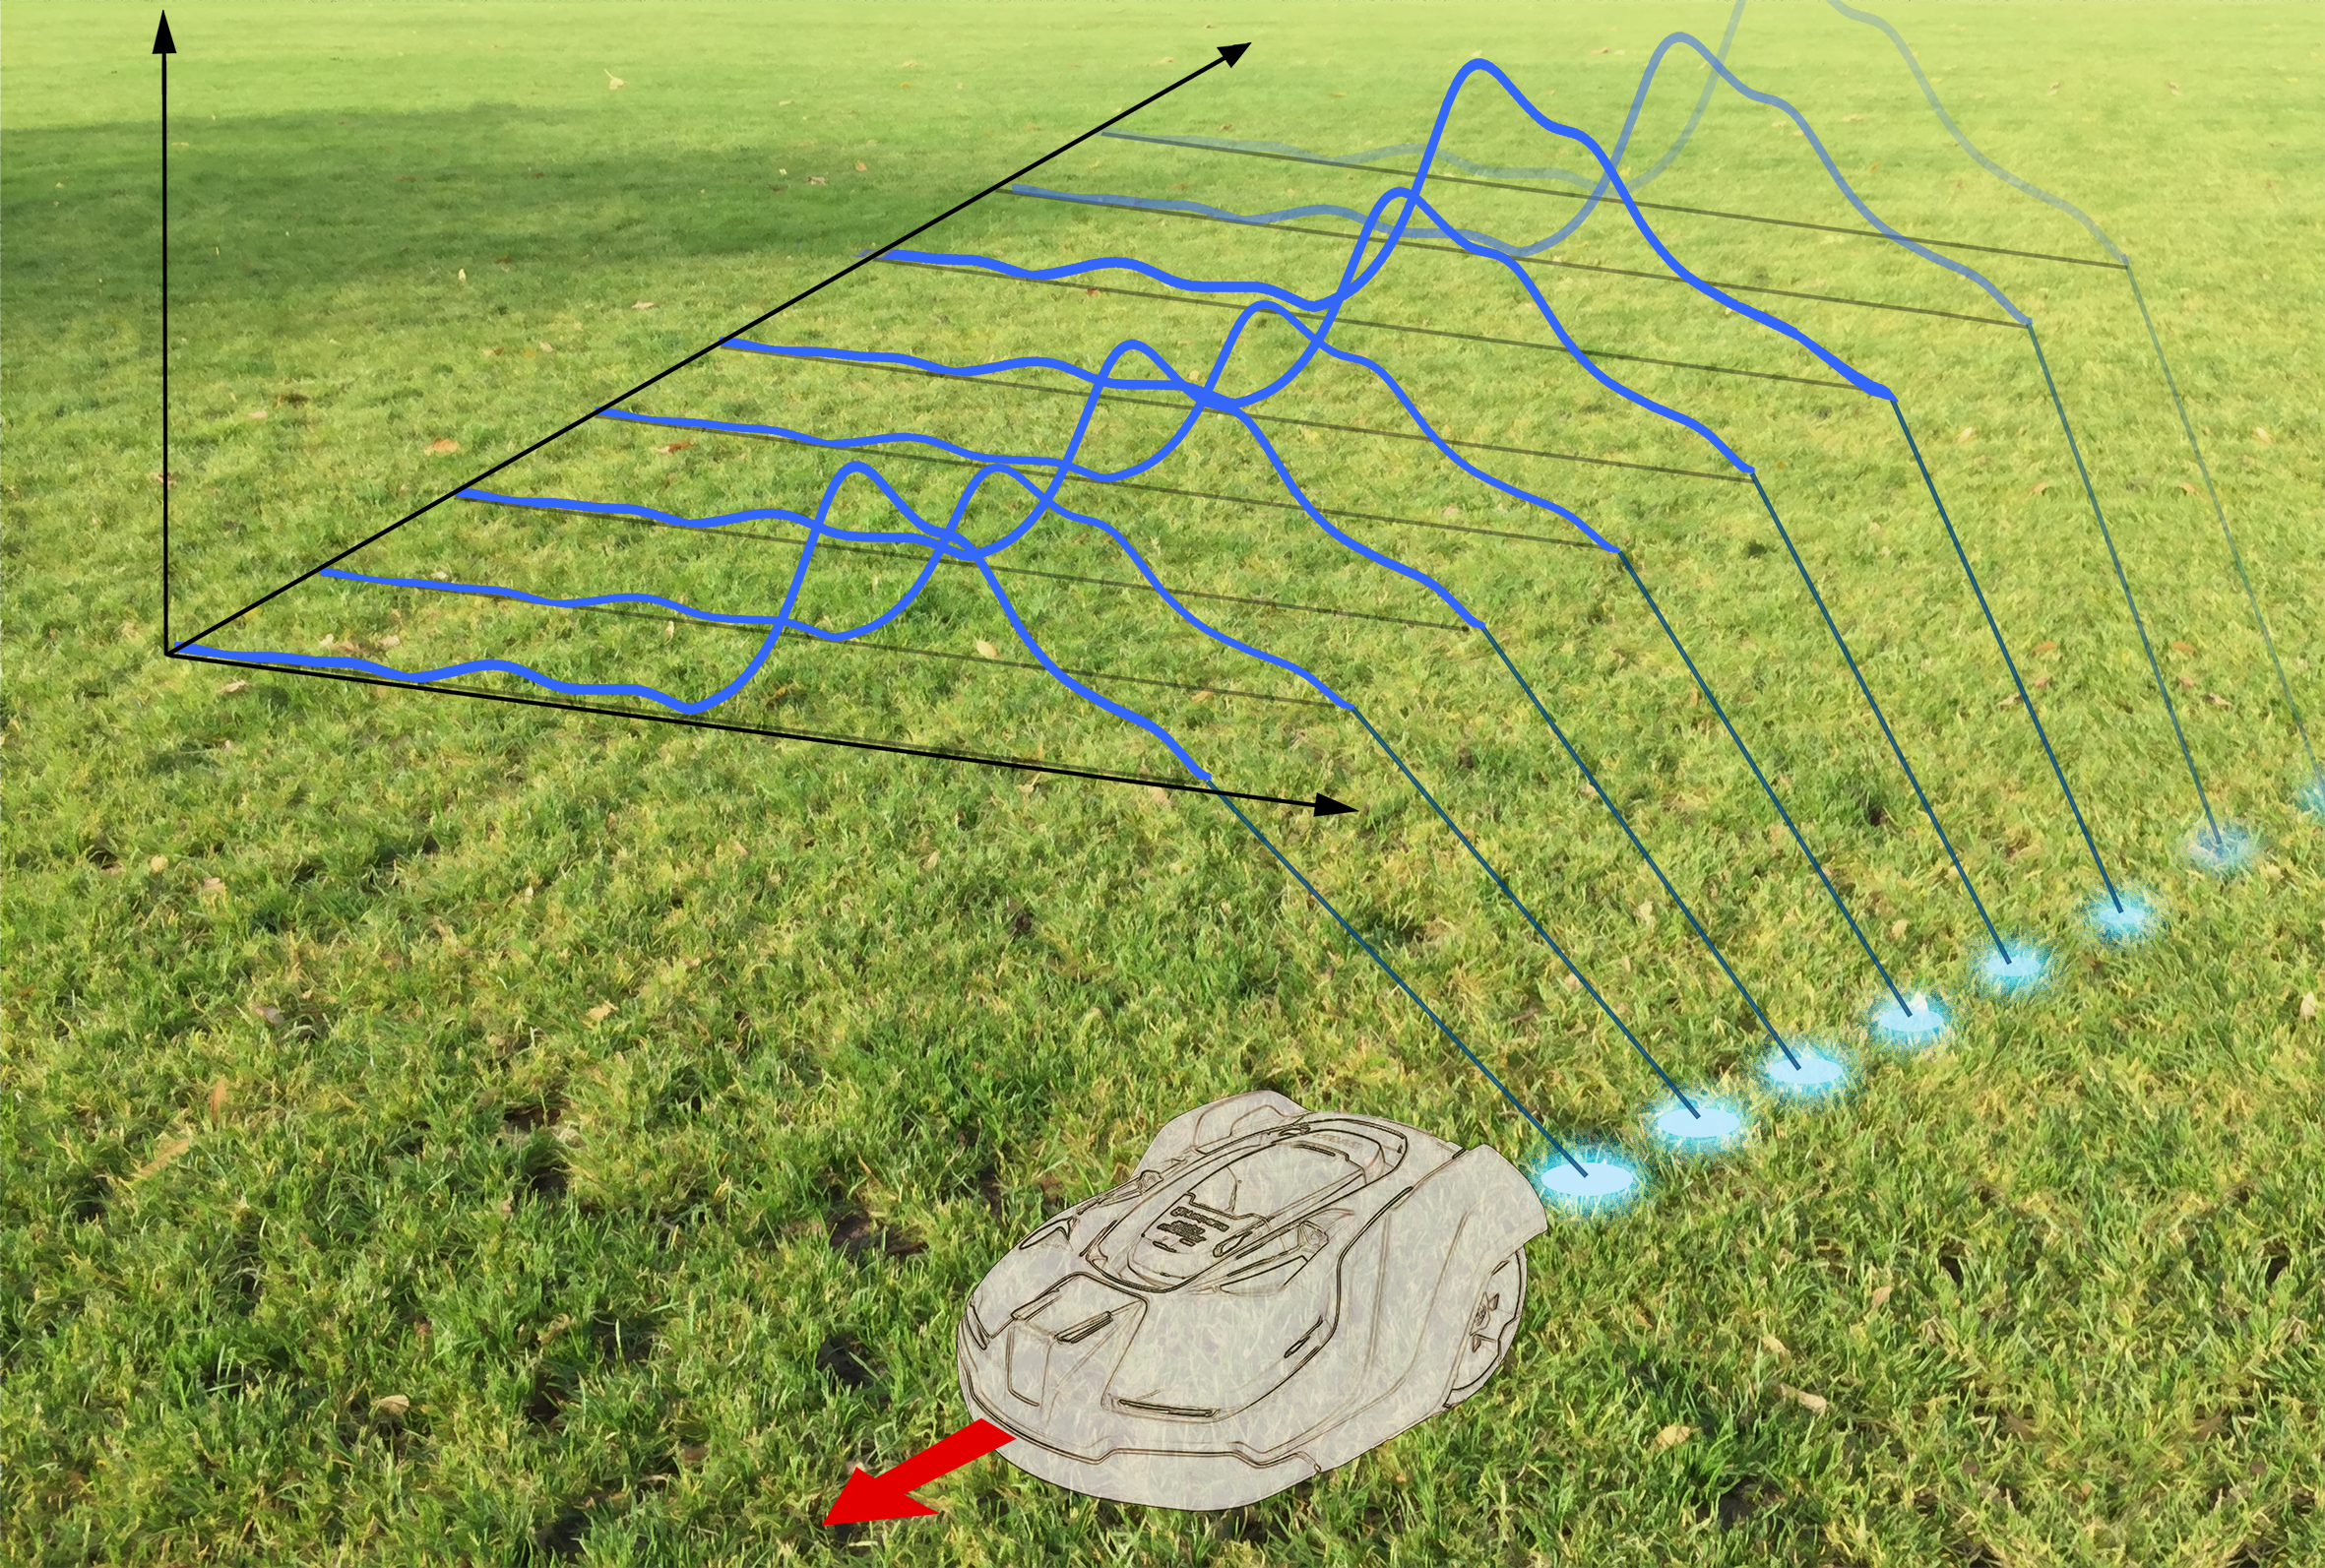
\includegraphics[scale=0.60]{figs_temp/data_collecting.jpg}
	\caption{Illustation of the data acquisition process. Radar sweeps are collected during constant velocity robot movement and stored in a data matrix. For visualization purposes, the absolute values of the complex radar sweeps are shown and the spatial distance between radar sweep measurements have been greatly exaggerated.}
	\label{fig:data_collecting}
\end{figure}

\section{Measurement Setup}\label{sec:setup}
As mentioned above, two sensors each capture one data matrix per measurement session. Sensor data is acquired while the robot is moving at a constant pace, as illustrated in Figure \ref{fig:data_collecting}. Furthermore, two mounting angles are used, where one sensor is facing directly towards the ground while the other has a $22.5^\circ$ forward tilt. The reasoning behind this setup is for each sensor to capture different aspects of the surface below; the sensor directed straight downwards may capture a larger component of the specular (i.e. mirror-like) reflection from the ground plane, while the tilted may capture more diffuse reflections. This concept is closely related to the surface ruggedness illustrated in Figure \ref{fig:reflections}. It is worth noting that the half power beam width of the sensor is roughly $60^\circ$ \citep{acconeer_datasheet_a111}, meaning that an angular width of about $60^\circ$ is illuminated by each sensor.

%It is worth noting that the half power beamwidth of the sensor is roughly $60^\circ$ \citep{acconeer_datasheet_a111}, meaning that each sensor illuminates about a $60^\circ$ angular width. %This idea is illustrated in figure \ref{fig:reflections}. If we are presented with two surfaces of the same material but with different ruggedness, the two will still scatter differently in spite of their equivalent dielectric properties. The scattering processes considered in this work should be highly dependant on the surface structure, where the predictability (or the randomness) should vary from material to material. 
\begin{figure}[h]
	\centering
	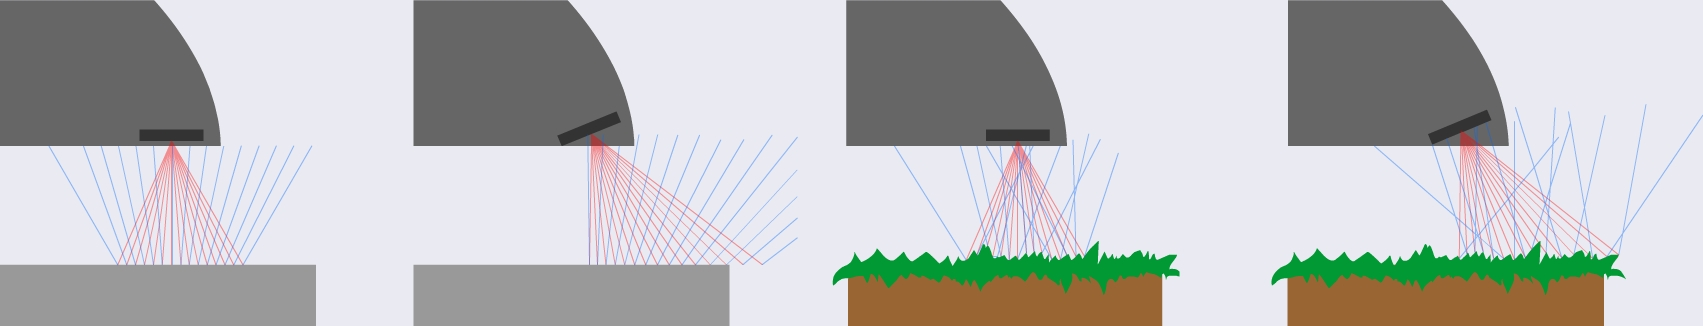
\includegraphics[scale=0.2]{figs_temp/reflections.jpg}
	\caption{By using two \gls{pcr} sensors with different mounting angles more diverse information about a target surface is obtained. The ratio between specular and diffuse reflectivity is dependent on surface roughness, as illustrated in the figure.}
	\label{fig:reflections}
\end{figure}

A final consideration is that as the sensors are placed on the inside of the robot plastic chassis, there is a risk for interference in the region between the plastic and the antenna. To avoid this, a small mount was 3D-printed so that the distance to the plastic was $\lambda_c/4$. Doing this means that any undesired wavelets propagating back and forth in this region interfere destructively due to the change in phase and the superposition principle of electromagnetic radiation \citep{griffiths_2018}.

\section{Target Surfaces}

In this work, we wish to see if we can create a binary classifier capable of distinguishing grass from non-grass surfaces. For the application of keeping a robot lawn mower in bounds, it is natural to select other surfaces that commonly border lawns. The selection of surfaces was made with this in mind, and is presented in table \ref{tab:count}, along with the number of measurement sessions per surface, each acquiring one data matrix with 50,000 slow time samples. Each session was taken either on a different day or in a different location than the rest. Note that the total sampling time amounts to\newline $50,000\cdot42/(F_s [\text{s}^{-1}]\cdot60)=175$ minutes.

\begin{table}[h]
	\centering
	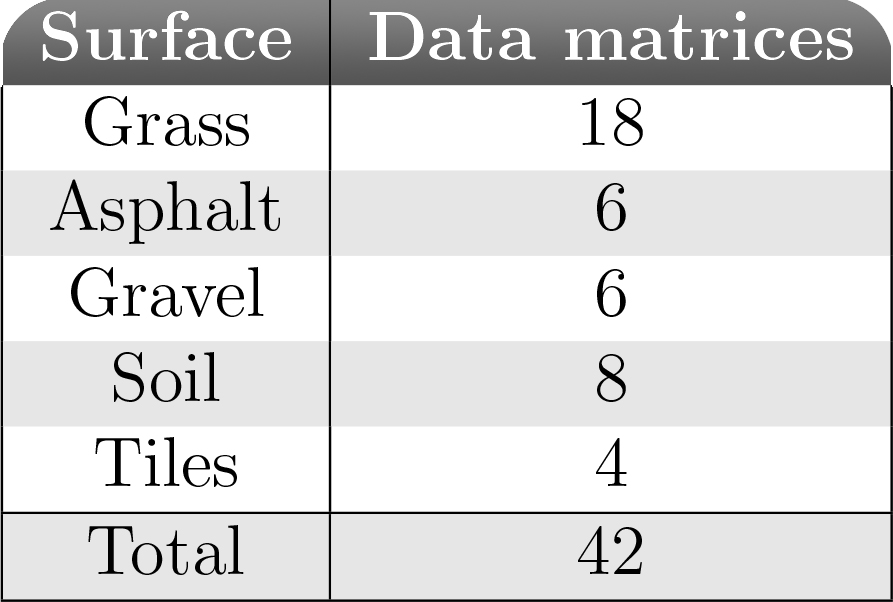
\includegraphics[scale=0.7]{figs_temp/table_surfaces.jpg}
	\caption{Measured surface types and number of captured data matrices per surface type.} 
	\label{tab:count}
\end{table}
%\begin{table}
%	\begin{center}
%		\begin{tabular}{|c|c|}
%			\hline
%			\rowcolor{gray!150}\color{white}\textbf{Surface} & \color{white}\textbf{Data matrices} \\
%			Grass & 18 \\
%			\rowcolor{gray!25} Asphalt & 6 \\
%			Gravel & 6 \\
%			\rowcolor{gray!25} Soil & 8 \\
%			Tiles & 4 \\ \hline
%			\rowcolor{gray!25} Total & 42 \\
%			\hline
%		\end{tabular}
%	\end{center}
%	\caption{Measured surface types and number of captured data matrices per surface type.}
%	\label{tab:count}
%\end{table}

\iffalse
\begin{table}
	\begin{center}
		\begin{tabular}{|c|c|}
			\hline
			\cellcolor{gray!150}\color{white}\textbf{Setting} & \cellcolor{gray!150}\color{white}\textbf{Value} \\
			Wavelet duration & 50 ps \\
			\cellcolor{gray!25}Sampling frequency & \cellcolor{gray!25}200 Hz \\
			Range swath & 7 to 23 cm \\ 
			\hline
		\end{tabular}	
	\end{center}
	\caption{Sensor settings.}
	\label{tab:sensor_settings}
\end{table}
\fi

\section{Measurement Settings}

The Acconeer \gls{pcr} system has several user-defined settings. In this section, a few key parameters of these are discussed, namely the range swath, the slow time sampling rate, and the wavelet duration. Although finding the appropriate sensor settings requires some level of trial-and-error due to hardware and software limitations, a good starting point can be found from a theoretical standpoint. 

\subsection{Sampling Rate}\label{sec:srate}
When working with radars and moving targets, it is important to select a sampling frequency, $F_s$, capable of resolving the maximum speed that an investigated target can attain. If the sampling frequency is too low, aliasing occurs, distorting the frequency spectrum \citep{lindgren_rootzezn_sandsten_2014}. In order to assure that aliasing does not occur, one must select a sampling rate at least twice the maximal frequency component received, $f_{max}$. This limit is commonly known as the Nyquist limit \citep{proakis_manolakis_1995}. From section \ref{sec:doppler} we find that the velocity, $v$, the carrier wavelength, $\lambda_c$ and the \gls{bf}, $f_d$ are related through $v \approx \lambda_cf_d/2$. Combining this result with the Nyquist limit, we require from the sampling rate that
\begin{equation}
	\label{eq:nyquist}
		F_{s} \geq 2f_{max} 
		= 2f_{d,max} 
		\approx \frac{4v_{max}}{\lambda_c}.
\end{equation}
\noindent
The maximum velocity, $v_{max}$, above is the \emph{radial} velocity. In the measurement setup depicted in Figure \ref{fig:sensor_placement}, a vehicle is moving forward at constant velocity, $v_0$, having a sensor mounted at the front with a 22.5-degree tilt and a 60 degree angular spread. The maximal velocity component that is orthogonal to the sensor occurs at the far end of the radar's view, at a $22.5^\circ + 30^\circ = 52.5^\circ$ tilt angle. With $\lambda_c=c/f_c=0.005$ m and the maximum orthogonal velocity component, $v_{\perp, max}$, the requirement above can be written as
\begin{equation}
	F_s \geq 
	\frac{4v_{\perp, max}}{\lambda_c}
	= \frac{4v_0\sin(52.5^\circ)}{\lambda_c} 
	\approx 190 \text{ Hz}.
\end{equation}
\noindent
Thus, in order to avoid aliasing, the sampling rate, $F_s$, should be at least 190 Hz. 


\begin{figure}[t]
	\centering
	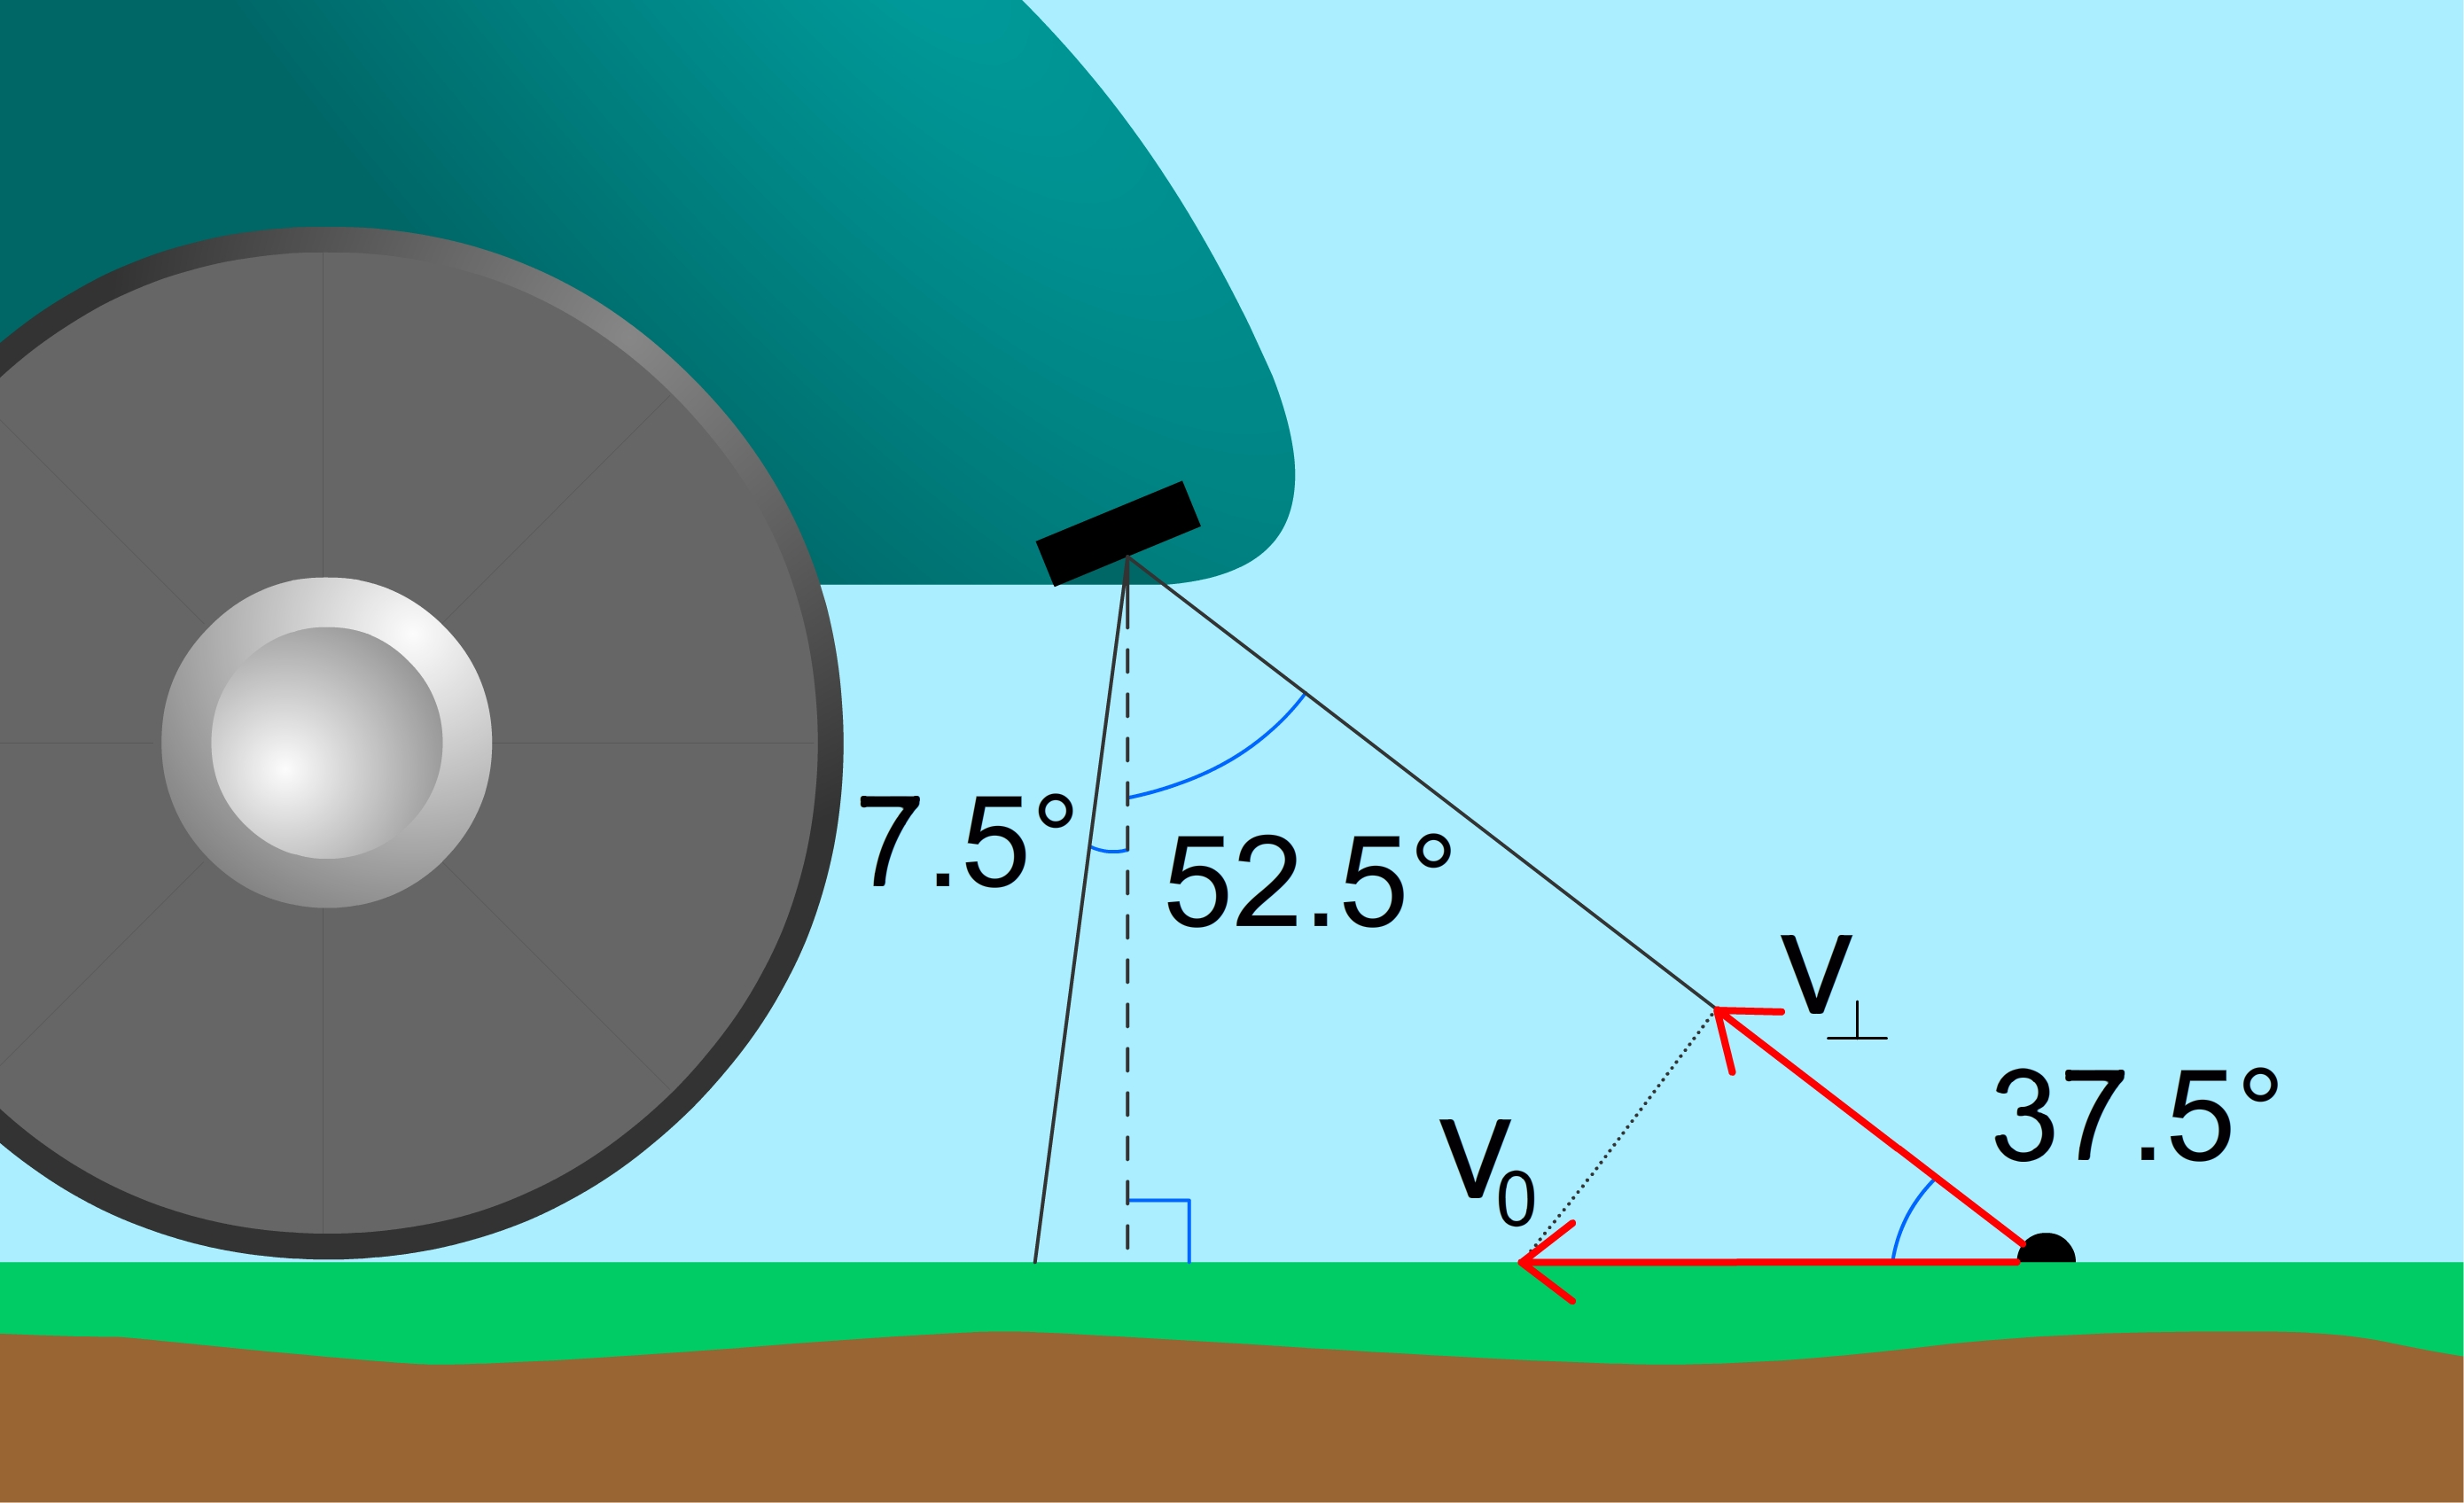
\includegraphics[scale=0.30]{figs_temp/sensor_placement.jpg}
	\caption{Sensor placement of the $22.5^\circ$-degree tilted sensor in the robot chassis. The figure indicates the furthest point visible by this sensor.}
	\label{fig:sensor_placement}
\end{figure}
\subsection{Wavelet Duration}

The length, or duration, of the transmitted wavelet pulses in a \gls{pcr} system determines the bandwidth. Taking a Fourier transform of a short wavelet produces a wider spectrum, and a longer pulse length conversely produces a narrower spectrum. Assuming the same amplitude, a longer wavelet corresponds to transmitting more energy and thus receiving a signal with better spectral resolution and \gls{snr}, while a shorter wavelet has better spatial resolution. Thus, the wavelet duration parameter becomes a tradeoff between spatial resolution and \gls{snr}. A reasonable strategy is therefore to start with a short wavelet and increase its duration until a reasonable \gls{snr} is obtained.  

\subsection{Range Swath}

Finally, the radar measures power over some range interval, also called the \emph{range swath} of the radar \citep{richards_2014}. Again, a tradeoff appears. If a short range swath is selected, we can increase the sampling rate and still stay within the allowed hardware transmission speed limitations. However, if the range swath becomes too short, we may miss useful information we could have collected outside the chosen interval. 

Thus, a reasonable strategy is to select the most critical interval and then increase the sampling frequency to its hardware allowed limit, keeping in mind that the sampling frequency should exceed the limit found above in section \ref{sec:srate}. As the distance to the surface plane is roughly 12 cm in the measurement setup, the furthest distance illuminated is $12/\sin(37.5^\circ)\approx 20$ cm from the sensor. We should therefore at least have a range swath spanning this region. 

The three settings for the three parameters discussed in this section are summarized in table \ref{tab:sensor_settings}.

\begin{table}
	\begin{center}
		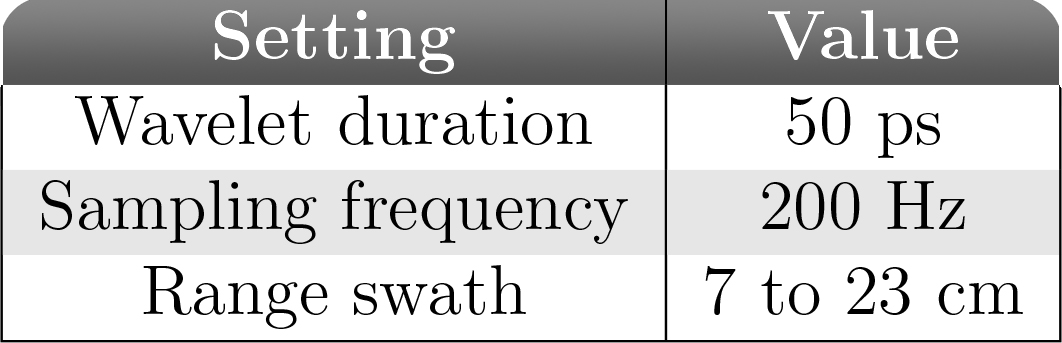
\includegraphics[scale=0.70]{figs_temp/table_settings.jpg}
	\end{center}
	\caption{Sensor settings. The wavelet duration is set as short as possible while maintaining a reasonable \gls{snr}.}
	\label{tab:sensor_settings}
\end{table}
%\begin{table}
%	\begin{center}
%		\begin{tabular}{|c|c|}
%			\hline
%			\cellcolor{gray!150}\color{white}\textbf{Setting} & \cellcolor{gray!150}\color{white}\textbf{Value} \\
%			Wavelet duration & Short \\
%			\cellcolor{gray!25}Sampling frequency & \cellcolor{gray!25}200 Hz \\
%			Range swath & 7 to 23 cm \\ 
%			\hline
%		\end{tabular}	
%	\end{center}
%	\caption{Sensor settings. The wavelet duration is set as short as possible while maintaining a reasonable \gls{snr}.}
%	\label{tab:sensor_settings}
%\end{table}

\section{Downsampling in Fast Time}
\label{downsampling}

% This part is cool but unncessary
%In information theory we interpret and quantify random variables by how unpredictable or unstructured observations of the random variables are \citep{anderson_johnnesson_2006}. Using such a framework, one could argue that variables that contain the same information as others in the same set are obsolete and can be discarded, as one ideally look for variables that contain information not found elsewhere in the set \citep{hyvasrinen_karhunen_oja_2004}.

Using the settings in table \ref{tab:sensor_settings}, we obtain 331 range samples per radar sweep in the 7-23 cm range swath, and as samples are equidistantly spaced, they are separated by $(230 \text{ [mm]}-70\text{ [mm]})/331\approx0.48$ mm. After examining a number of radar sweeps, it is clear that closely spaced points are highly related, and that including all datapoints for analysis is redundant. This correlation occurs in part due to \gls{iq} demodulation, as it involves low pass filtering in fast time (see appendices), making closely spaced points highly correlated. With this redundancy of information in mind, we may downsample by some integer factor, $D$, without significant loss of information. Downsampling measurements $r_1(d,t)$ and $r_2(d,t)$ by a factor $D$ can be expressed as
\begin{equation}
	\label{eq:downsamp}
	r_{1,D}(d, t) = r_{1}(dD,t),
	\quad \text{and} \quad r_{2,D}(d,t) = r_{2}(dD,t)
\end{equation}
and the data matrix $r_D(n,t)$ is formed correspondingly.

\section{Sweep Normalization}\label{sec:norm}

One hardware quirk of the radar sensors used in this project is that their gain, found in $A_r$ in the \gls{rre}, can vary significantly from one sensor to the next. This means that faced with the same target at the same distance, two sensors exhibit a similar sweep structure, but possibly with a different scaling. Assuming a model's training data has been collected with one sensor, it could therefore be difficult to successfully perform classifications with the same model using a sensor which has a different gain. A way to overcome this issue is to perform radar sweep normalization as a preprocessing step. There are multiple ways of performing such a normalization. %This is due to the fact that a linear scaling difference between two sensors behaves nonlinearly in the prediction output, due to nonlinearities both in the feature extraction process as well as in the classification process.

A simple strategy is to simply divide each sweep with its maximum absolute value. While this may intuitively seem like a good idea, it eliminates signal evolution structures between consecutively captured sweeps - if neighboring sweeps vary in received signal strength, we wish to capture such a behavior. A better solution is to instead have the normalization method depend on several consecutive sweeps. Normalizing using multiple sweeps thus maintains some of the relative amplitude structure. Constructing a smaller gain independent data matrix, $x(n,t)$, consisting of $K$ downsampled sampling points and $T$ consecutive sweeps, starting from slow time sample, $T_m$, we can normalize by the average amplitude through
\begin{equation}
	x(n,t) = 
	\frac{r_D(n, T_m + t)TK}{\sum_{n=0}^{K-1}\sum_{\tau=0}^{T-1}|r_D(n, T_m+\tau)|}.
\end{equation}
\noindent
Thus, we can perform gain normalization while, at least partially, maintaining any structures or patterns present in the returning sweep energy. The drawback of this normalization is that information pertaining to absolute measurements of target surfaces' \gls{rcs} is lost in the process.

